\RequirePackage{silence}
\WarningFilter{scrbook}{Usage of package `fancyhdr'}  % Hepthesis issues
\WarningFilter{scrbook}{Usage of package `tocbibind'} % Hepthesis issues
\WarningFilter{biblatex}{File }  % Bei Gelegenheit gegenprüfen!
\WarningFilter{tocbasic}{`tocbibind' redefinition of `\listoffigures'}
\WarningFilter{tocbasic}{`tocbibind' redefinition of `\listoftables'} 
\WarningFilter{chktex}{You should perhaps use `\min' instead.} % unfortunately -
\WarningFilter{chktex}{You should perhaps use `\max' instead.} % - doesn't work
\WarningFilter{latex}{Marginpar on page} % due to todonotes
\WarningFilter{LaTeX}{Command }
\documentclass{akdai}
% debugging
%\usepackage{lua-visual-debug}
% \usepackage{endfloat}
% wondering how to fix obscure errors? try preceding \protect

% Language-Encoding und Font
\usepackage{polyglossia}        % Alternative zu Babel
\usepackage{csquotes}           % Required by Polyglossia
\setmainlanguage[variant=british]{english}
\setotherlanguage[babelshorthands=true]{german}

% Citation, Verweise
\usepackage[style=ieee,backend=biber]{biblatex}
\addbibresource{BibLaTex/zotero.bib}
\addbibresource{BibLaTex/citavi_db.bib}
\usepackage{verbatimbox}
\usepackage{fancyvrb}
\usepackage[style=base]{caption}
\usepackage{listings}           % refer to 'minted vs. texments vs. verbments'
\usepackage{xcolor}
\usepackage{hyperref}           % Verlinkungen im Dokument
\hypersetup{
 colorlinks,
 linkcolor={red!45!black},
 citecolor={blue!50!black},
 urlcolor={blue!80!black}
}
\usepackage{nameref}
\usepackage{booktabs}           % Tabellenpaket-keine vertikal und dicken Linien
\usepackage[inline,shortlabels]{enumitem}
\usepackage[acronym]{glossaries}		% \gls{<golssary-entry>}
\setacronymstyle{long-short}
\usepackage{cleveref}
\lstset{
  frame=single,
  columns=fullflexible,
  literate={-}{-}1
}

\lstnewenvironment{python}[1][]{
  \definecolor{commentsColor}{rgb}{0.497495, 0.497587, 0.497464}
  \definecolor{keywordsColor}{rgb}{0.000000, 0.000000, 0.635294}
  \definecolor{stringColor}{rgb}{0.558215, 0.000000, 0.135316}
  \lstset{
    float=h,
    backgroundcolor=\color{white},                % choose the background color; you must add \usepackage{color} or \usepackage{xcolor}
    basicstyle=\footnotesize,                     % the size of the fonts that are used for the code
    breakatwhitespace=false,                      % sets if automatic breaks should only happen at whitespace
    breaklines=true,                              % sets automatic line breaking
    captionpos=b,                                 % sets the caption-position to bottom
    commentstyle=\color{commentsColor}\textit,    % comment style
    deletekeywords={},                            % if you want to delete keywords from the given language
    escapeinside={\%*}{*)},                       % if you want to add LaTeX within your code
    extendedchars=true,                           % lets you use non-ASCII characters; for 8-bits encodings only, does not work with UTF-8
    frame=tb,	                   	                % adds a frame around the code
    keepspaces=true,                              % keeps spaces in text, useful for keeping indentation of code (possibly needs columns=flexible)
    keywordstyle=\color{keywordsColor}\bfseries,  % keyword style
    language=Python,                              % the language of the code (can be overrided per snippet)
    otherkeywords={},                             % if you want to add more keywords to the set
    numbers=left,                                 % where to put the line-numbers; possible values are (none, left, right)
    numbersep=5pt,                                % how far the line-numbers are from the code
    numberstyle=\tiny\color{commentsColor}\noncopynumber,       % the style that is used for the line-numbers
    rulecolor=\color{black},                      % if not set, the frame-color may be changed on line-breaks within not-black text (e.g. comments (green here))
    showspaces=false,                             % show spaces everywhere adding particular underscores; it overrides 'showstringspaces'
    showstringspaces=false,                       % underline spaces within strings only
    showtabs=false,                               % show tabs within strings adding particular underscores
    stepnumber=1,                                 % the step between two line-numbers. If it's 1, each line will be numbered
    stringstyle=\color{stringColor},              % string literal style
    tabsize=2,                                    % sets default tabsize to 2 spaces
    title=\lstname,                               % show the filename of files included with \lstinputlisting; also try caption instead of title
    columns=fullflexible,                         % Using fixed column width produces nice alignment. I think it's ugly, though -> fullflexible
    literate={-}{-}1
             {*}{*}1
             {\ }{{\copyablespace}}1 {\ \ }{{\copyablespaceTwo}}1,
    #1                                            % Optional arguments
    }  
  }{} 

% Fonts
\usepackage{fontspec}
\usepackage{unicode-math} % fontspec wird auch von unicode-math geladen?
%\setmainfont{Times New Roman} % set fontsize: 11p
%\setmainfont{TeX Gyre Pagella} % set fontsize: 12p
%\setmathfont[ItalicFont=*, BoldFont=*]{TeX Gyre Pagella Math}

% Math-Packages und Fonts
\usepackage{physics} % ||norm|| und |abs|
\usepackage{amsmath}
\usepackage{mathrsfs} % für \mathscr

% Theoreme und Definitionen
\usepackage{amsthm}
\theoremstyle{definition}
\newtheorem{definition}{Definition}[section]

% Formatierung
\usepackage{geometry}           % Paket für Zeilenabstand 
\usepackage{setspace}           % Paket für Zeilenabstand 
\usepackage{microtype}


% Subsections
\setcounter{secnumdepth}{5}
\setcounter{tocdepth}{5}

% Fileinsertion
\usepackage{pdfpages}           % Paket zum Einfügen von PDFs

% Sonstiges                     % Einfügen von Grafiken
\usepackage{graphicx}
\usepackage{subcaption}         % Replacement for subfig package which is broken
\graphicspath{ {./pictures/} }
\usepackage{xcolor}
\usepackage[normalem]{ulem}     % Unterstreichen von Text mit \uline
\usepackage[de-DE]{datetime2}   % Kalenderdaten in deutschem Format
\usepackage{blindtext}          % Repräsentativer als Lorem Ipsum
\usepackage{kantlipsum}         % Cooler als blindtext
\setlength{\marginparwidth}{2cm}
\usepackage[textwidth=15mm]{todonotes} % Einfügen von Todos, Option: [disable]
\usepackage[shortcuts]{extdash} % \=/ for nonbreaking dash
\usepackage{url}
\crefname{const}{constraint}{constraints}
\usepackage{xifthen}
\usepackage{xargs}
\usepackage{array,tabularx}

%%%%% Workarounds %%%%%
\setlength{\marginparwidth}{2cm} % without: trouble with todonotes

\newcommand*\appendixmore{ % add title to Abstract
  \addsec{\appendixname}%
  \renewcommand{\thesubsection}{\Alph{subsection}}%
}

% list of listings title
\renewcommand*{\lstlistlistingname}{List of listings}

% Make Python-Listing line numbers uncopyable
\usepackage[space=true]{accsupp}
\newcommand{\noncopynumber}[1]{%
    \BeginAccSupp{method=escape,ActualText={}}%
    #1%
    \EndAccSupp{}%
}
% Fix spaces in Python listing (really necessary?)
\newcommand{\copyablespace}{\BeginAccSupp{method=hex,unicode,ActualText=00A0}\ \EndAccSupp{}}
\newcommand{\copyablespaceTwo}{\BeginAccSupp{method=hex, unicode, ActualText=00A000A0}\ \ \EndAccSupp{}}
\makeatletter
  \def\lst@Literatekey#1\@nil@{\let\lst@ifxliterate\lst@if
  \expandafter\def\expandafter\lst@literate\expandafter{\lst@literate#1}}
\makeatother

%%%%% /Workarounds %%%%%

%%%%% Custom Commands %%%%%
% Math Equation Parameter description environment:
\newenvironment{conditions}
  {\par\vspace{\abovedisplayskip}\noindent
   \tabularx{\columnwidth}{>{\(}l<{\)} @{}>{\({}}c<{{}\)}@{} >{\raggedright\arraybackslash}X}}
  {\endtabularx\par\vspace{\belowdisplayskip}}
%%%%% /Custom Commands %%%%%


\author{
	Malte Zietlow, Finn Wellershaus \\ 
	\\
	Nordakademie\\ 
	Köllner Chaussee 11\\ 
	25337 Elmshorn \\ 
	malte.zietlow@nordakademie.de \\
	finn.wellershaus@nordakademie.de
}
\makeglossaries{}             % makeglossaries <document-root ohne .tex> per cmd

\begin{document}

\title{Introduction to Many-to-Many Mimical Puppetry and its Detection}
\maketitle

\listoftodos{}            % Aktuelle ToDo-Notes

% Acronyms and glossaries

% ----------------------------- Acronyms -----------------------------
\newacronym{nn}{NN}{Neural Network}
\newacronym{ai}{AI}{Artificial Intelligence}
\newacronym{cnn}{CNN}{Convolutional Neural Network}
\newacronym{gan}{GAN}{Generative Adversarial Network}
\newacronym{lrcn}{LRCN}{Long-Term Recurrent Convolutional Neural Network}
\newacronym{lstm}{LSTM}{Long Short-Term Memory}
\newacronym{rnn}{RNN}{Recurrent Neural Network}
\newacronym{auc}{AUC}{Area under the Curve}
\newacronym{dsp-fwa}{DSP-FWA}{Dual Spatial Pyramid-Face Warp Artifacts}

% ----------------------------- Glossary Entries -----------------------------

\newglossaryentry{redditor}{name={redditor},description={a contributor to the
webpage \url{https://www.reddit.com}}}

\newglossaryentry{path}{
    name={path},
    description={A path \(P_{i, j}\) exists between two neurons \(i, j\) if the value of \(i\) is fed into \(j\).},
}

\newglossaryentry{message}{
    name={message},
    description={Messages are defined in \fullref{subsubsect:message-notation}}
}


% Frontmatter
% \begin{abstract}
    In this paper we give a theoretical overview of methods for replicating a
    generic content manipulation technique named \textit{DeppFake}. Our focus
    lies on providing a mathematical formulation and giving a technical demo of
    it.
\end{abstract}

% Mainmatter
\section{Introduction}
In late 2017, \gls{redditor} \textit{deepfake} began publishing pornographic footage
on \url{https://www.reddit.com/r/deepfakes}, where he replaced the actors' faces
with those of celebrities --- without their consent. As a consequence, he
received increased media coverage in early 2018, after the release of a first 
article and interview on vice-motherboard~\cite{Cole.2017}. While he coined the
term \textit{DeepFake} for face-\textit{replacement} and face-\textit{reenactment}
technologies, both were already actively researched in academia with research 
dating back to at least 1997~\cite{Bregler.1997}.
Following this, there was an increased awareness for \textit{DeepFakes} which also
caused more research to be conducted, from \(3\) papers published in \(2017\) to
more than \(150\) in \(2018-2019\)~\cite{mirsky_creation_2020} as well as
resulting in first government action~\cite{senate_-_homeland_security_and_governmental_affairs__house_-_energy_and_commerce_deepfake_2019}.

\par
The aim of this paper is
\begin{enumerate*}[a.)]
    \item to give the reader an introduction to the process of creating manipulated
    images via the generic content manipulation technique named \textit{DeepFake}
    and
    \item to give an overview on different approaches to the detection of such manipulated footage.
\end{enumerate*}

\subsection{Structure}
In the remainder of this section, the limitations to the scope of this paper are
presented. Then, in \cref{sect:background}, an overview and definition of \textit{DeepFakes}
is given, including also a discussion of ethical challenges.
This is followed by a summary of the creation of many-to-many \textit{DeepFakes}
in \cref{sect:creation-of-deepfakes}. Finally, different methods of detecting
\textit{DeepFakes} can be found in \cref{sect:detection}.

\subsection{Limitations}\label{subsect:limitations}
While there are multiple \textit{flavors} of \textit{DeepFakes} (see \cref{subsubsect:deepfake-flavors}),
this study explicitly works within the scope of many-to-many mimical puppetry and its
detection. This means that neither \textit{DeepFakes} of text or audio signals,
face-replacement or body reenactment are part of this work. This is mainly
due to spatial constraints and considering that in their core principles the techniques are mostly
similar. Beyond that, one-to-one and one-to-many \textit{DeepFakes} (see \cref{subsubsect:generalizability-deepfakes})
are not examined. This restriction is made because we consider many-to-many \textit{DeepFakes}
to be of greater risk due to their more generic nature and thus larger applicability.
\todo{unify all the sources, no duplications}
\section{Background}\label{sect:background}

\subsection{DeepFakes and CheapFakes}
In this work, a distinction between the so called CheapFakes and \textit{DeepFakes}
is made. On the one hand, CheapFakes are produced by using contemporary video 
and picture editing software. The name CheapFake should under no circumstance be
interpreted as an assessment of their effectiveness since they can still be used
to effectively fool users. An example of this usage might be a video of US House
Speaker Nancy Pelosi which was slowed down for her to appear drunk\todo{add reference}.
On the other hand, \textit{DeepFakes} describe the results of machine-learning
algorithms, which are most often a form of or combination of \glspl{nn}.
The names simply refer to the different levels of sophistication of the different
approaches. Arguably, at some point, they might even merge together with editing 
software utilizing machine learning more and \textit{DeepFake} technology becoming
accessible and integrated into existing tooling.

\subsection{Flavors of DeepFakes}\label{subsubsect:deepfake-flavors}
Broadly, \textit{DeepFakes} can be sorted into two categories, as described by~\textcite{Mirsky.2020}:
There is a source \textit{s} and a target \textit{t}

\begin{description}
    \item[Face Reenacment] Here, the expression of \textit{s} is used to drive
    the expression of \textit{t}~\cite{Mirsky.2020}. The source is
    therefore also called driver \textit{d}.
    \item[Replacement] In this case, some part of \textit{t} is replaced
    by the corresponding part of \textit{s}. An example would be the swapping of
    \textit{t}'s face with the one from \textit{s}, preserving \textit{t}'s mimic.
\end{description}

\subsection{Generalizability of Generative Models for DeepFakes}\label{subsubsect:generalizability-deepfakes}
In the design of \glspl{nn} for the creation of \textit{DeepFakes}, one must choose
the range of targets to which it is applicable~\cite[cf.][]{Mirsky.2020}:
\begin{description}
    \item[one-to-one] after training, the approach is applicable only to a
    single target and source/driver;
    \item[many-to-one] after training, the approach is applicable only to a
    single target, but arbitrary sources/drivers;
    \item[many-to-many] after training, the approach is applicable both to
    arbitrary targets and sources/drivers.
\end{description}
As mentioned in \cref{subsect:limitations}, only \textbf{many-to-many} approaches
are presented in this paper because they are more generic than \textbf{one-to-one} or
\textbf{many-to-one}.

\subsection{Ethical Challenges}
The importance of \textit{DeepFake} detection in conjunction with the ethical
challenges which arise from the use of this technology. The ability to create
arbitrary fake images bears multiple risks for misuse. Firstly, there is the
aspect of misinformation and propaganda. For example by showing images or videos
of political candidates saying things they have not said and that can incriminate
them. Moreover, another aspect to take into consideration would be pornography,
since it is possible to change faces to other people's bodies, which can lead to
non-consensual pornography. Following these dimensions, there are two types of attacks: to public or political figures and to private individuals. The first category
is defined by attackers having more resources at hand for an attack, e.g.\ an
organized action against a specific political candidate. The second category, in 
contrast, is defined by the attackers' lack of adequate resources, e.g.\ an angry 
ex-boyfriend. Even though the second category might pose a real risk since not 
that much effort might be needed to spread a basic amount of false information, in the 
end, the attacker's capabilities are somewhat limited. However, changes in the ease of use and 
availability of \textit{DeepFake} technologies can affect its uses towards targeting
private individuals.
\section{Creation of DeepFakes}\label{sect:creation-of-deepfakes}
Statistical models come in multiple classes with divergent properties.
Two such classes are discriminative and generative models. Generative models
learn the statistical properties of the input domain~\cite[cf.][\nopp{}651\psqq]{Goodfellow.2016}.
For example, they are able to generate unique images of human faces, based on
previously observed ones~\cite{Karras.2019}.

\par
Generative models are thus the focus of techniques for creating DeepFakes. As
this serves as an introduction to the creation of DeepFakes, we limit the scope
to:
% Description of basic network types
\begin{description}[leftmargin=0cm]
    \item[\glspl{ed}] \glspl{ed} consist of at least two networks, \gls{en} and
    \gls{de} (see \cref{subfig:ed}). The \gls{en}-part is trained to extract
    useful features \(\text{En}(x)=e\). This is often done by narrowing
    layer-width towards its center or some other regularization criterion~\cite[cf.][499-505]{Goodfellow.2016}.
    After encoding \(x \rightarrow e\), \(e\) is fed into \gls{de} to arrive at
    the final result \(\text{De}(e)=x_g\). \Glspl{ae} are a special form of
    \gls{ed}, where the network is trained to reproduce its inputs, i.e.\
    \(\text{De}(\text{En}(x))\approx x\).

    \item[\glspl{gan}] \glspl{gan} like \gls{ed} consist of at least two networks,
    \gls{gen} and \gls{disc} (see \cref{subfig:gan}). In a sense, \gls{gen} can
    be interpreted similar to the \gls{de} part of the \gls{ed}. But instead of
    relying on \gls{en} to extract features \(\text{En}(x)=e\), the input
    \(z,\ \text{G}(z)=x_g\) is sampled from a so called prior-distribution
    \(z\sim p_z\), e.g.\ the normal distribution \(p_z=\mathcal{N}(0, 1)\). Then,
    using \(z\), \gls{gen} generates images \(\text{G}(z)=x_g\). \Gls{disc} on
    the other hand tries to discern whether an input is from the original face
    \(x\sim X\) or generated by \gls{gen} \(x_g\). By training \gls{gen} and
    \gls{disc} are then trained alternation, such that \gls{gen} tries to fool
    \gls{disc} into thinking that \(x_g\) is an image from the target and \gls{disc}
    trying to discern correctly between \(x\sim X\) and \(x_g\sim \text{G}(p_z)\).
    That way we are able to generate realistically looking faces similar to that
    of the target~\cite{Goodfellow.2014}.
\end{description}
% Figure of basic network types
\begin{figure}[h]
    \centering
    \subcaptionbox{\label{subfig:ed}}{
        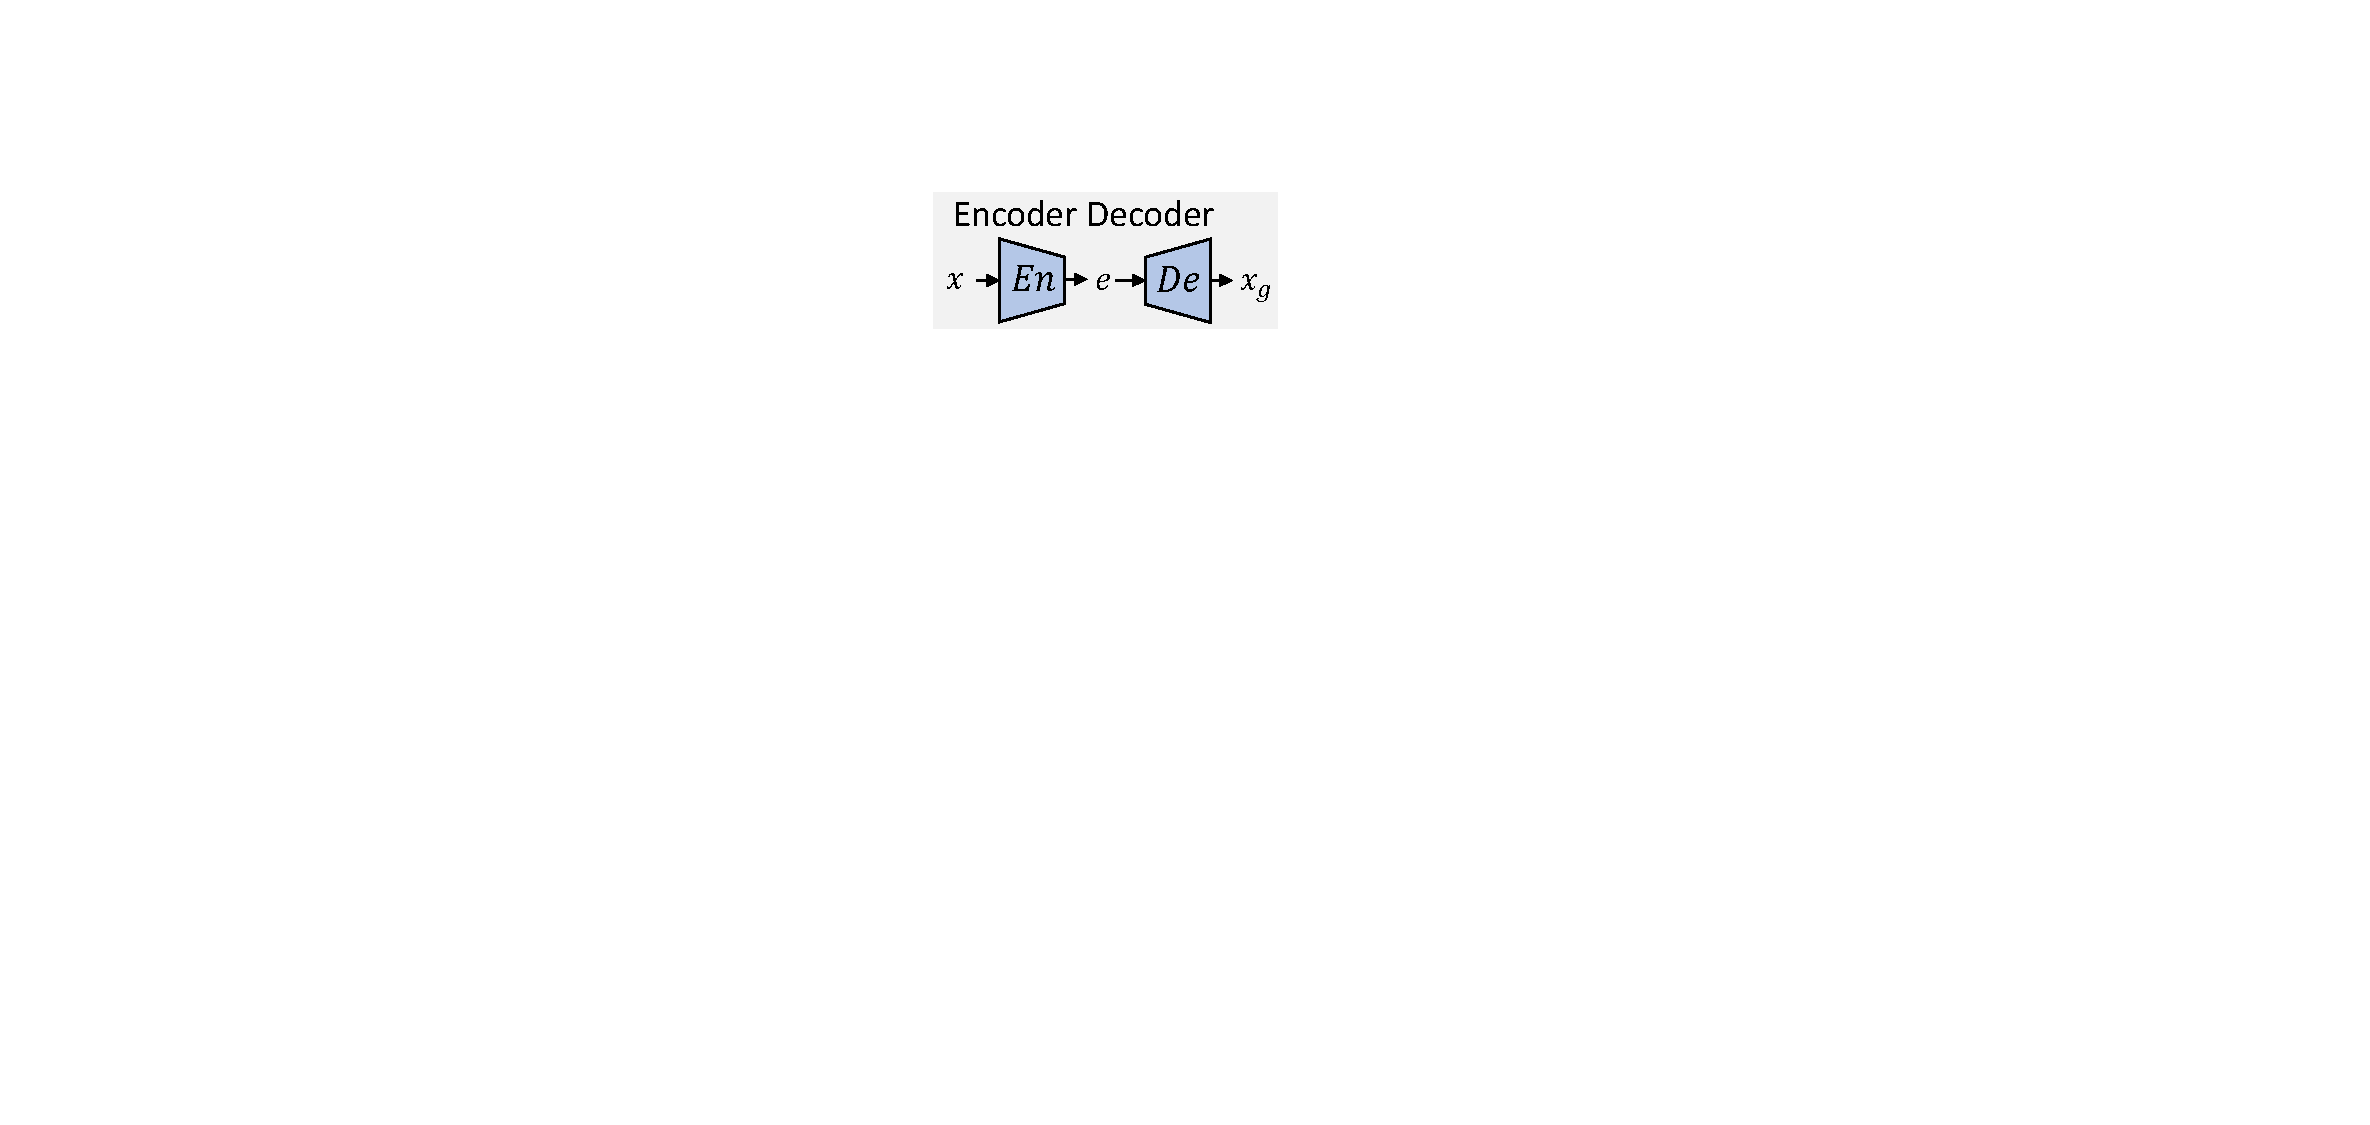
\includegraphics[width=3.3cm]{nns_ed.pdf}
    }
    \subcaptionbox{\label{subfig:gan}}{
        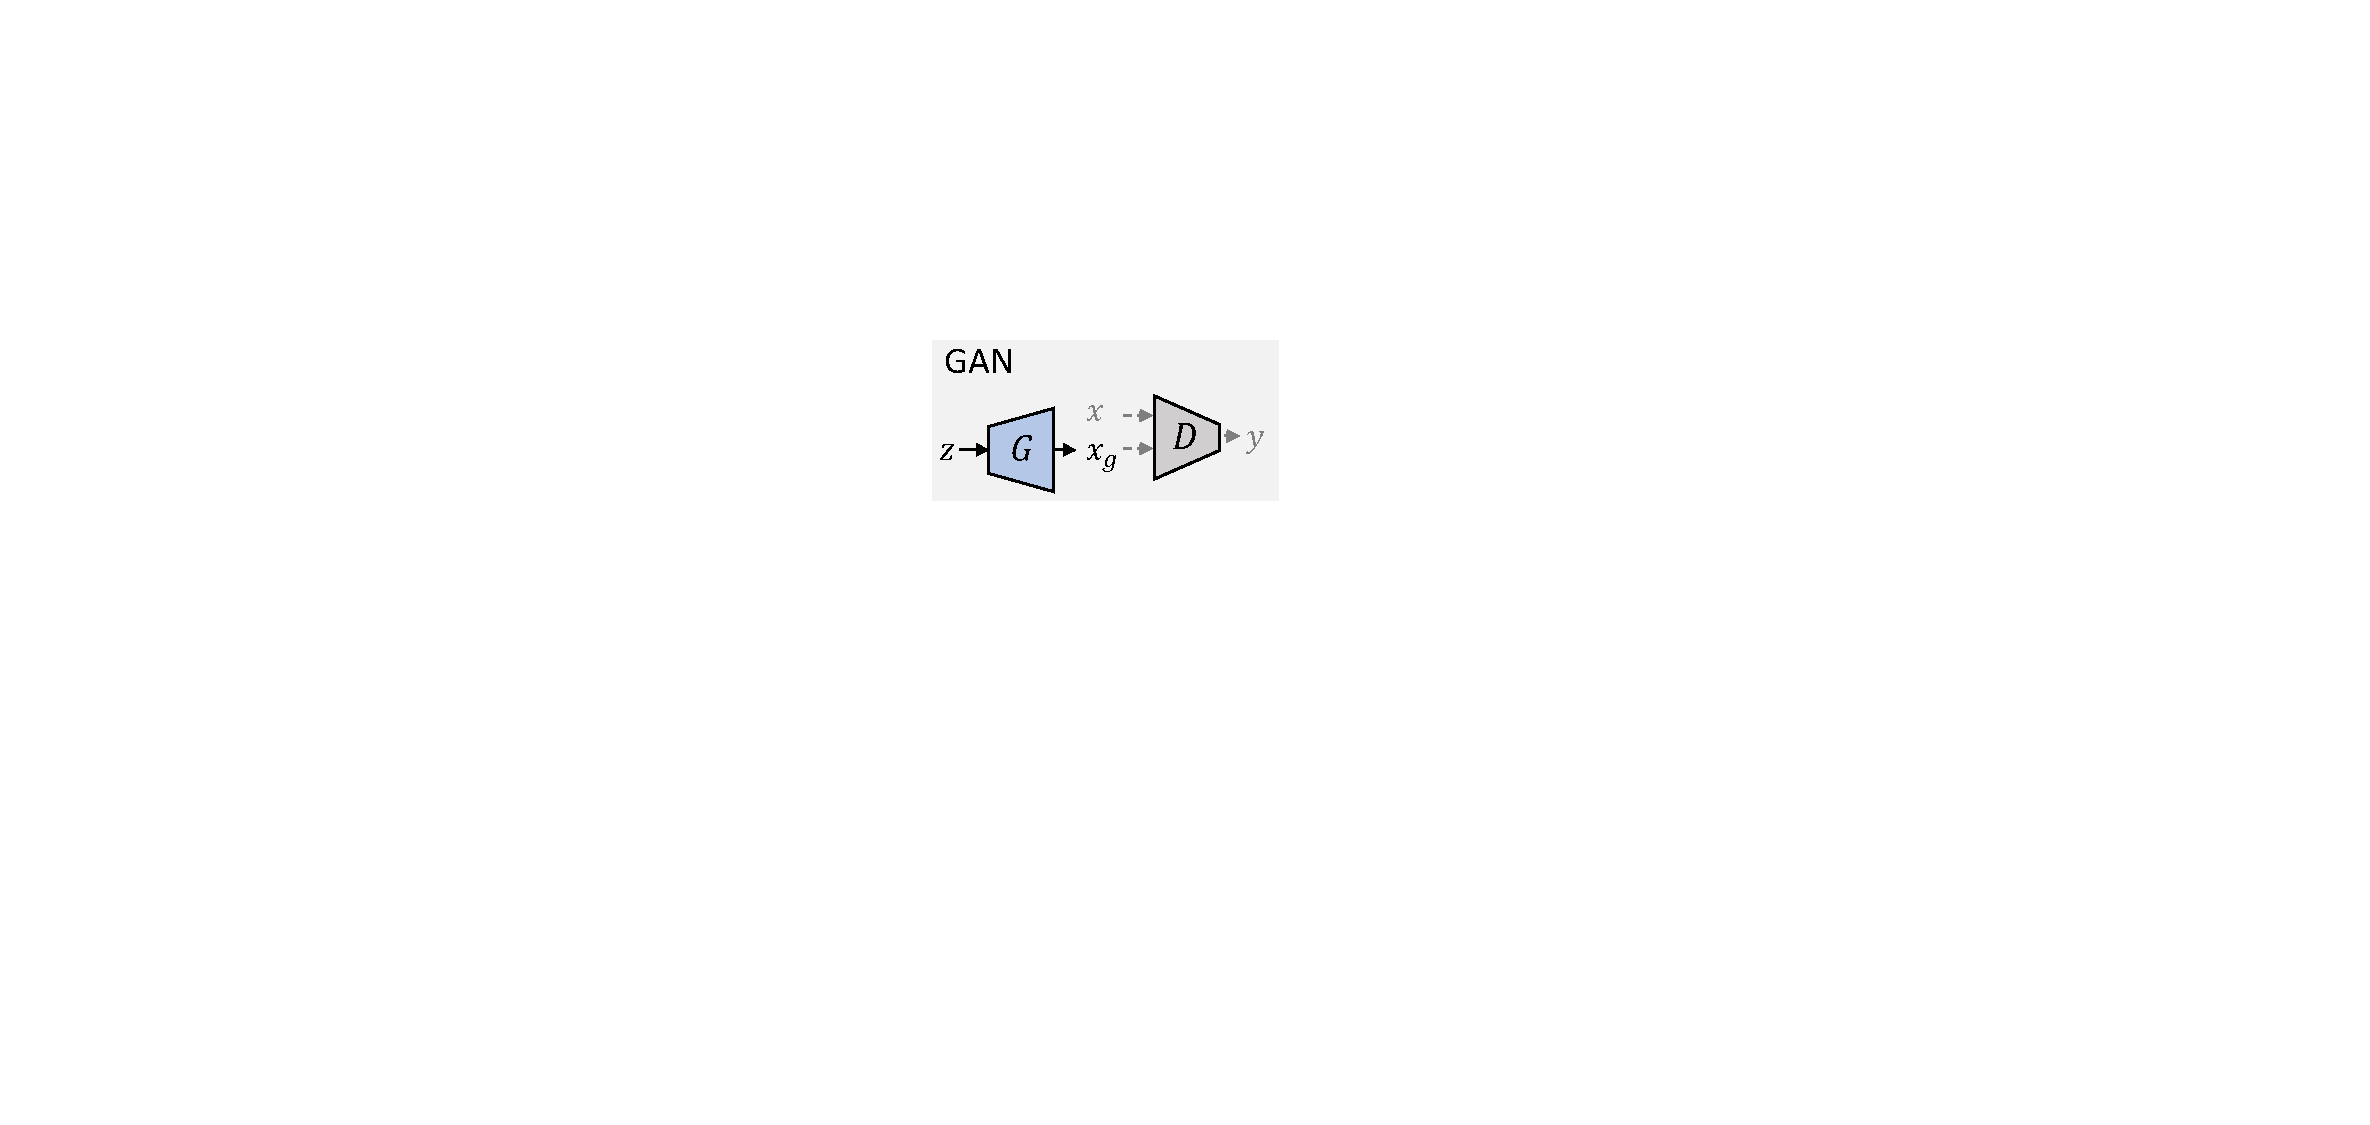
\includegraphics[width=3cm]{nns_gan.pdf}
    }
    \subcaptionbox{}{
        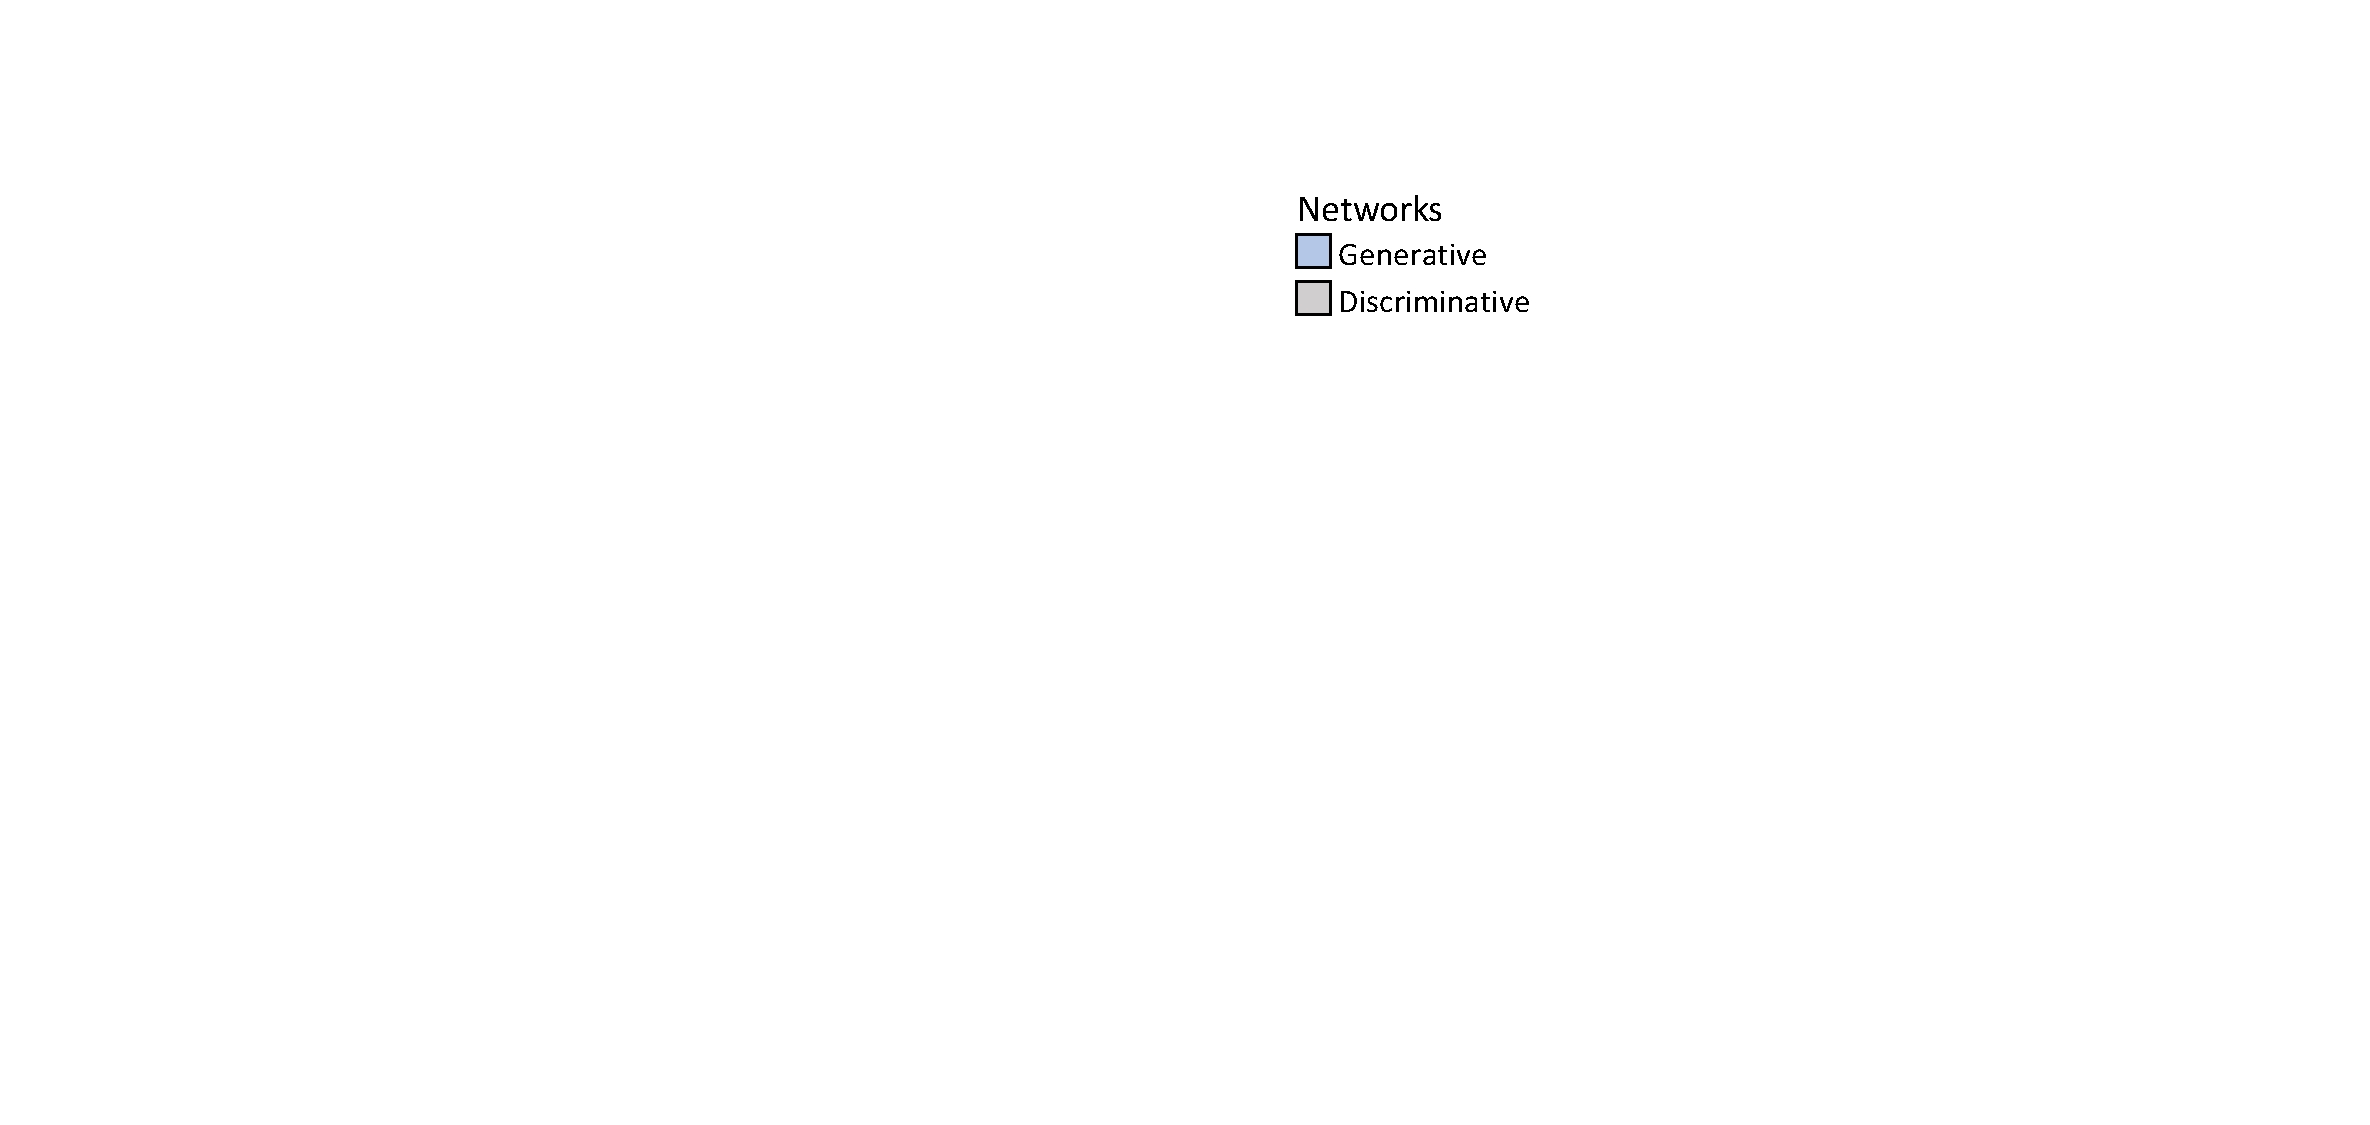
\includegraphics[width=2.5cm]{nns_description.pdf}
    }
    \caption{Selection of generative models, adopted from~\cite{Mirsky.2020}}\label{fig:generative-models}
\end{figure}

When trying to create believable mimical puppetry, there are three \textbf{goals}
we try to reach in final image \(x_g\):\todo{explain that \(x_t:target,\ x_d:driver\) and so on}
\begin{enumerate}[1.)]
    \item we try to preserve the mimic of \(x_d\) in \(x_g\), s.t.\ \(\text{mimic}(x_d)=\text{mimic}(x_g)\)\label{goal:mimic-perservation}
    \item we try to preserve the identity target \(x_t\) in \(x_g\), s.t.\ \(\text{id}(x_t)=\text{id}(x_g)\)\label{goal:preserve-identity}
    \item we try to generate a realistically looking image\label{goal:increase-realism}
\end{enumerate}
\subsection{Generating an image at all}
We can take these goals and construct a model after them. In order to generate
an image we utilize the \gls{ed}-model from \cref{subfig:ed}

\subsection{Preserving Mimic}
To tackle goal~\ref{goal:mimic-perservation}, one must define how to
numerically represent the mimic of a face, \(\text{mimic}(x)=\mathord{?}\).
Two such representations are
\begin{enumerate*}[a.)]
    \item facial landmarks or
    \item \gls{facs}
\end{enumerate*}
For simplicity, only \gls{facs} is considered. A discussion of facial landmarks
can be found in e.g.\ \cite{Ha.2020}

\paragraph*{Facial Action Coding System (FACS)}
The \gls{facs} was introduced in 1978 by \textcite{Ekman.1978}. They grouped
muscle regions of the face to 58 so called \glspl{au} which can be represented
by vectors. A major advantage of \glspl{au} over facial landmarks is that they
are (more or less) invariant (i.e.\ the same expression is encoded similarly)
between faces, head angle and scale~\cite{Pham.2018}.

\par
Following this discussion, \gls{facs} is used. \Glspl{au} might be computed using
a generic \gls{aue}, e.g.\ \cite{Senechal.2015}. The \gls{au}-vectors are then
concatenated to the encoded representation (\(\text{En}(x_t)=e\)) and used in
the \gls{de}-step. To enforce goal~\ref{goal:mimic-perservation}, the difference
in \glspl{au} between final DeepFake \(\text{AUE}(x_g)=a_g\) and driver
\(\text{AUE}(x_d)=a_s\)\todo{decide driver or source} are minimized in training:
\(\min{(\left|a_g-a_s\right|)}\). A visualization of this is given in \cref{fig:gath-aue}.
\begin{figure}[htp]
    \center{}
    \vspace{-1em}
    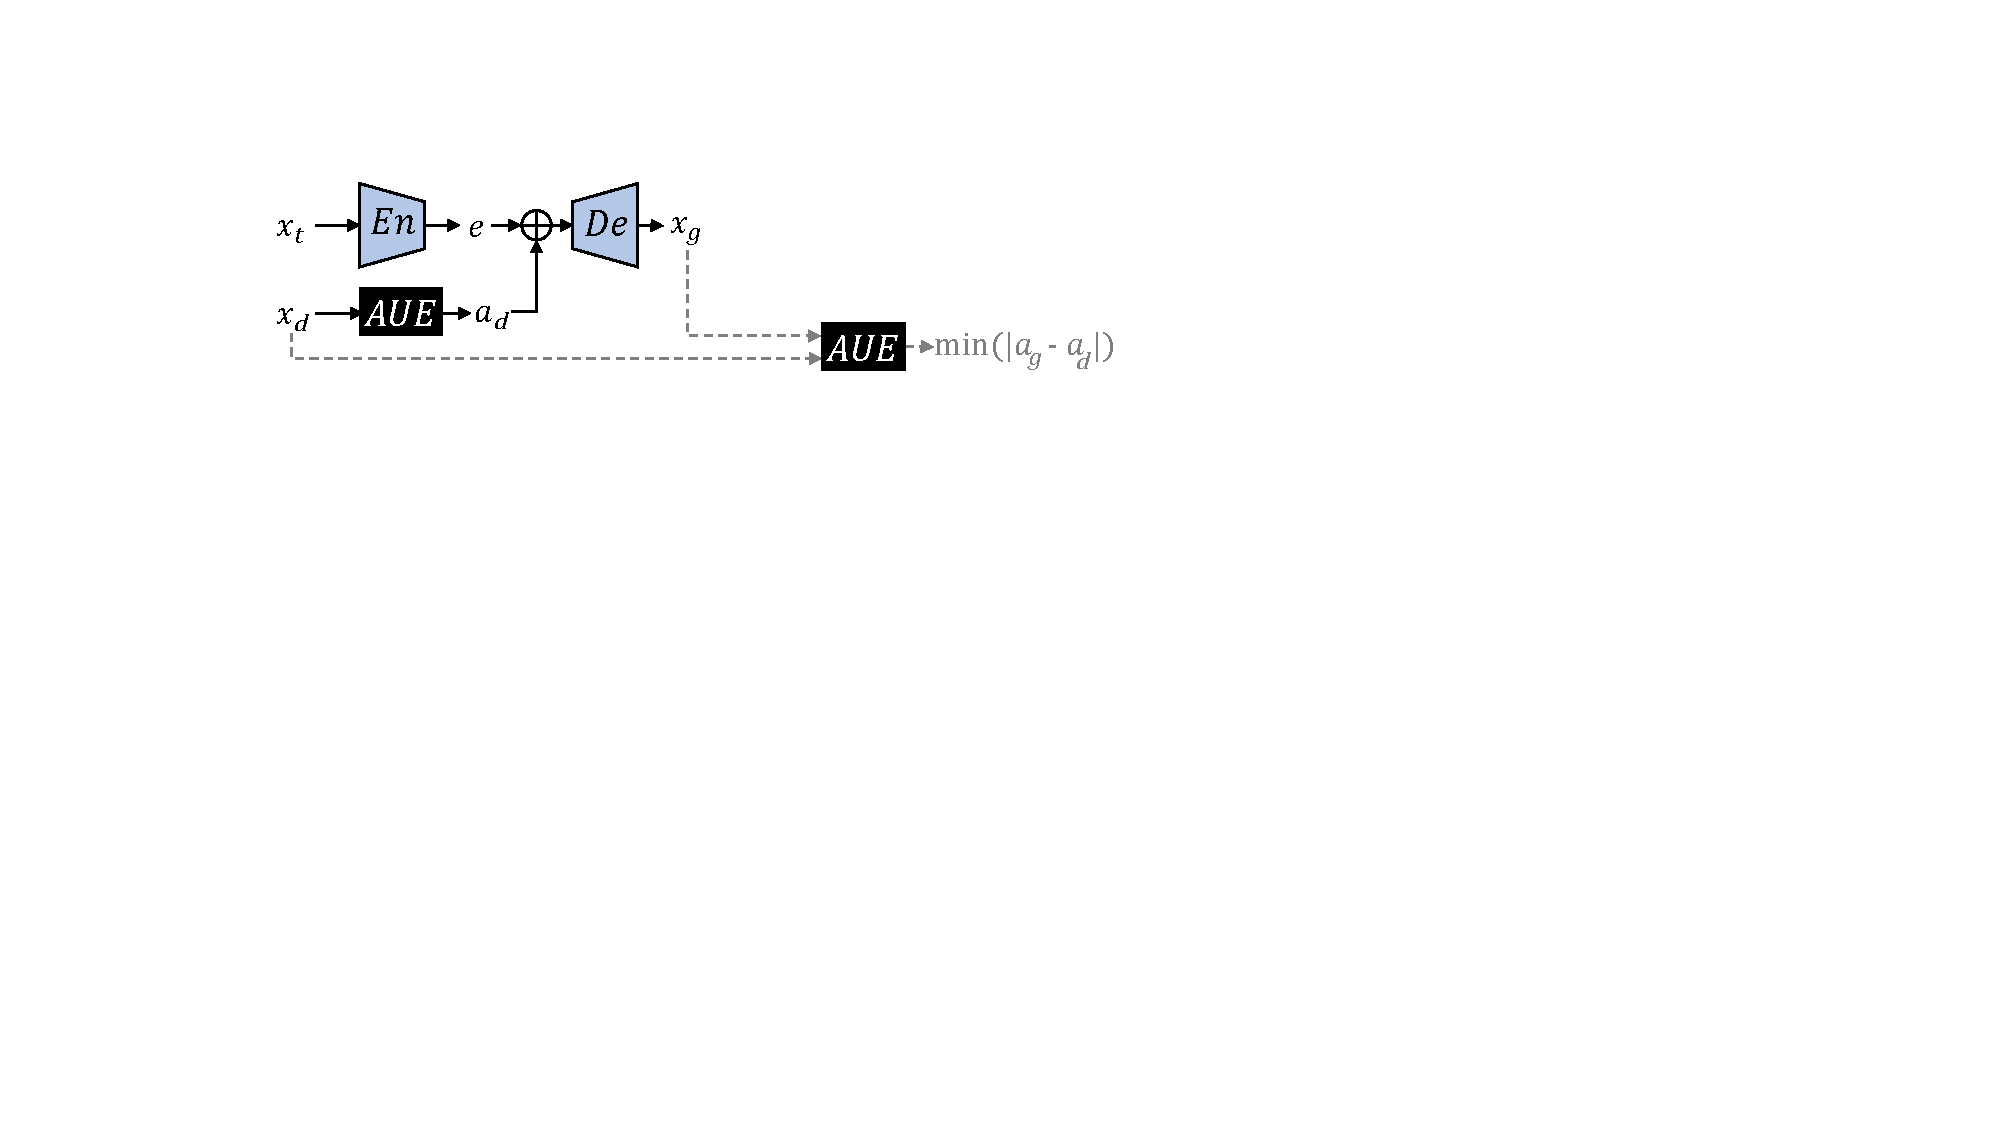
\includegraphics[width=.65\textwidth]{gath_aue.pdf}
    \caption{\gls{ed}-architecture enriched with \glspl{au}, where \(\bigoplus\)
    denotes concatenation. Grey paths are used solely in training, inspired
    by~\cite{Mirsky.2020, Pham.2018}}\label{fig:gath-aue}
    \vspace{-1em}
\end{figure}

\subsection{Preserving Identity}
Training the model on preserving the identity of the target requires a training
set of known targets, e.g.\ \cite{Chen.2015,Cao.2014,Tarres.2011} consisting of 
about 2000 identities~\cite{Pham.2018}. One can then learn an image classifier
\(I\), e.g.\ MobileNet~\cite{Howard.2017} (for its simplicity and speed) to
assign the correct identity to a given image. Once the classifier \(I\)
converges, it can be added to the training procedure of the model, minimizing
the cross-entropy identity loss \(\mathcal{L}_{id}\) (see \cref{eq:identity-loss}).
A visualization of this is given in \cref{fig:gath-aue-id}.
\begin{figure}[htp]
    \vspace{-1em}
    \center{}
    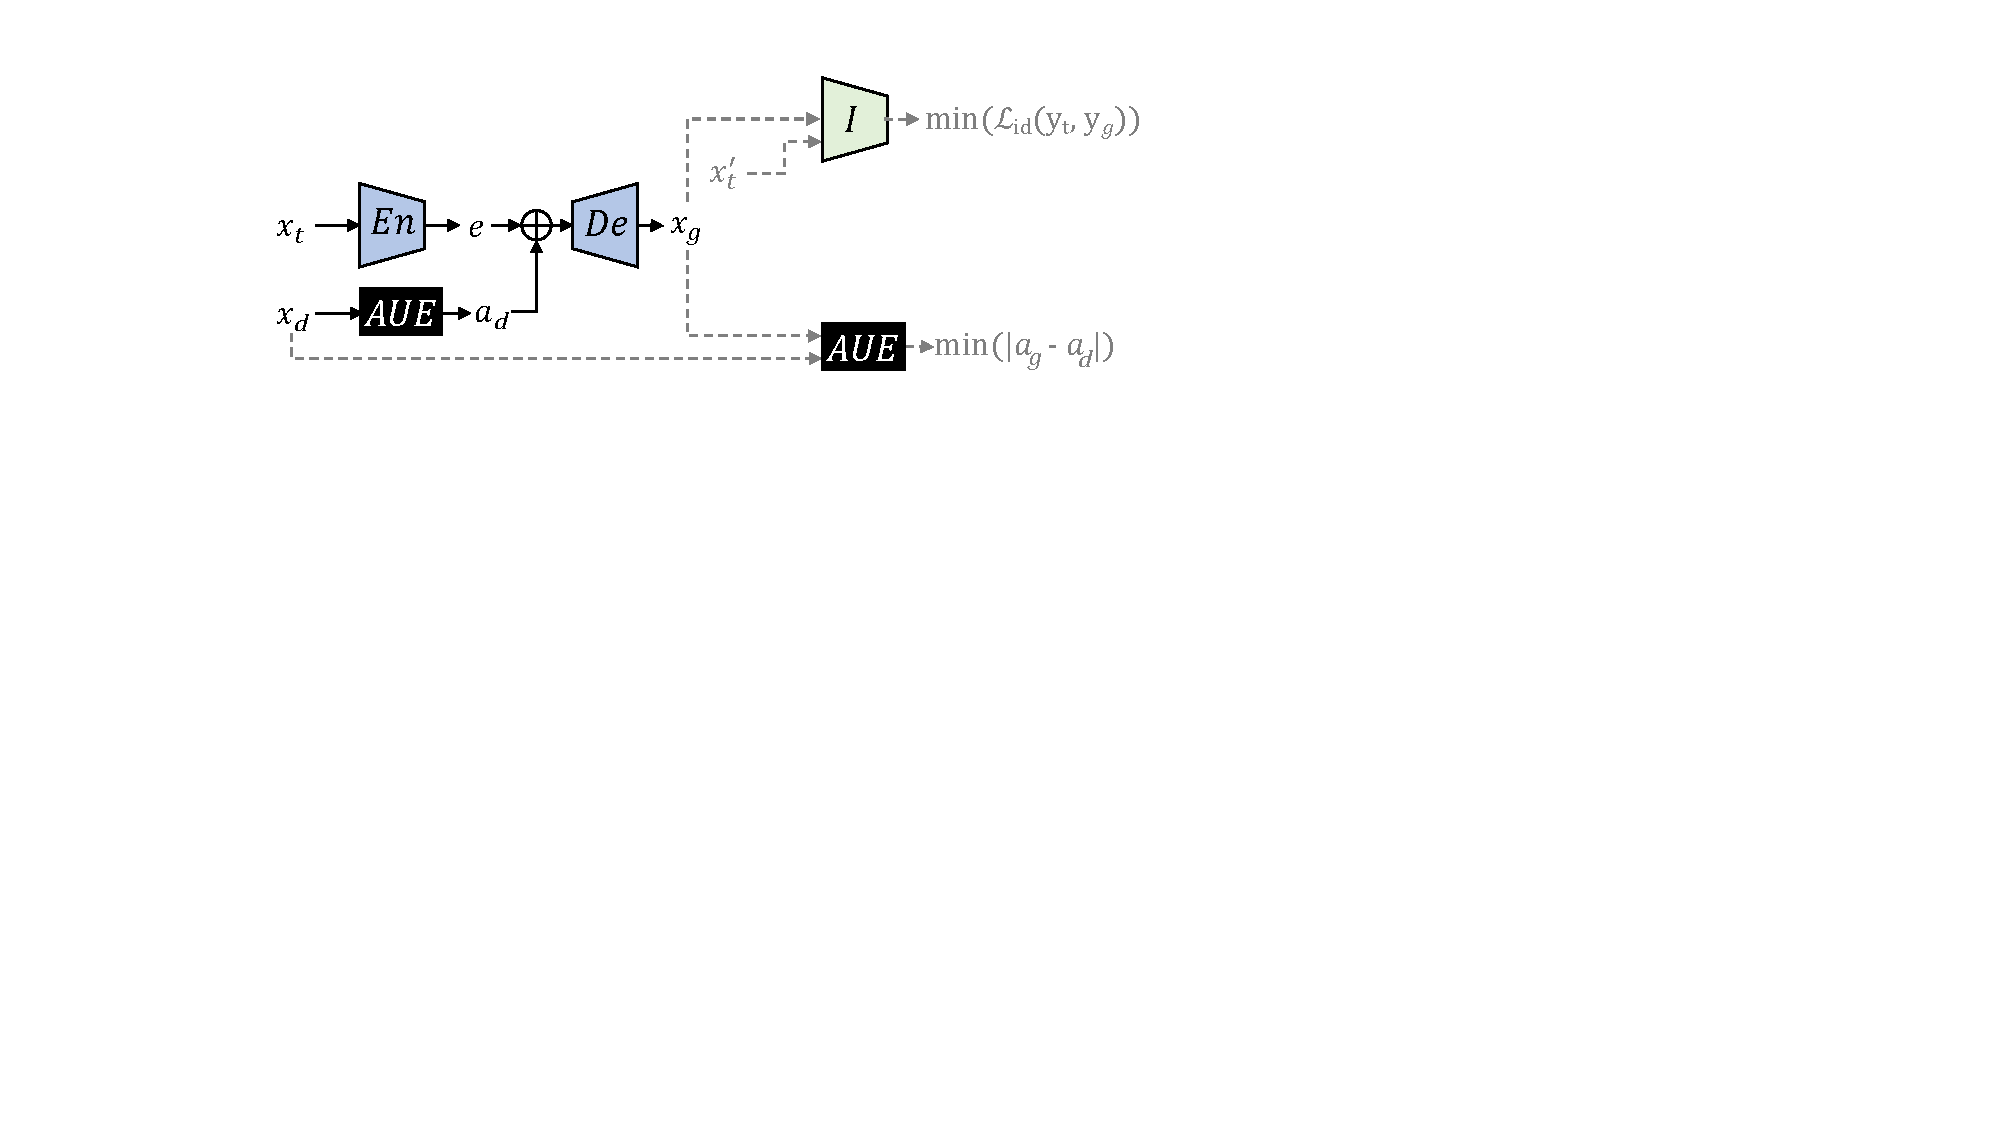
\includegraphics[width=.6\textwidth]{gath_aue_id.pdf}
    \caption{\gls{ed}-architecture enriched with \glspl{au} and an identity
    constraint, where \(\bigoplus\) denotes concatenation, \(x'_t\) is a randomly
    chosen image with identity of the target \(t\). Grey paths are used solely
    in training, inspired by~\cite{Mirsky.2020, Pham.2018}}\label{fig:gath-aue-id}
    \vspace{-1em}
\end{figure}

\subsection{Increasing Realism}
Finally to increase realism (goal~\ref{goal:increase-realism}), a \gls{gan}-inspired
discriminator \gls{disc} (see \cref{subfig:gan}) is adopted.
\begin{figure}[htp]
    \vspace{-1em}
    \center{}
    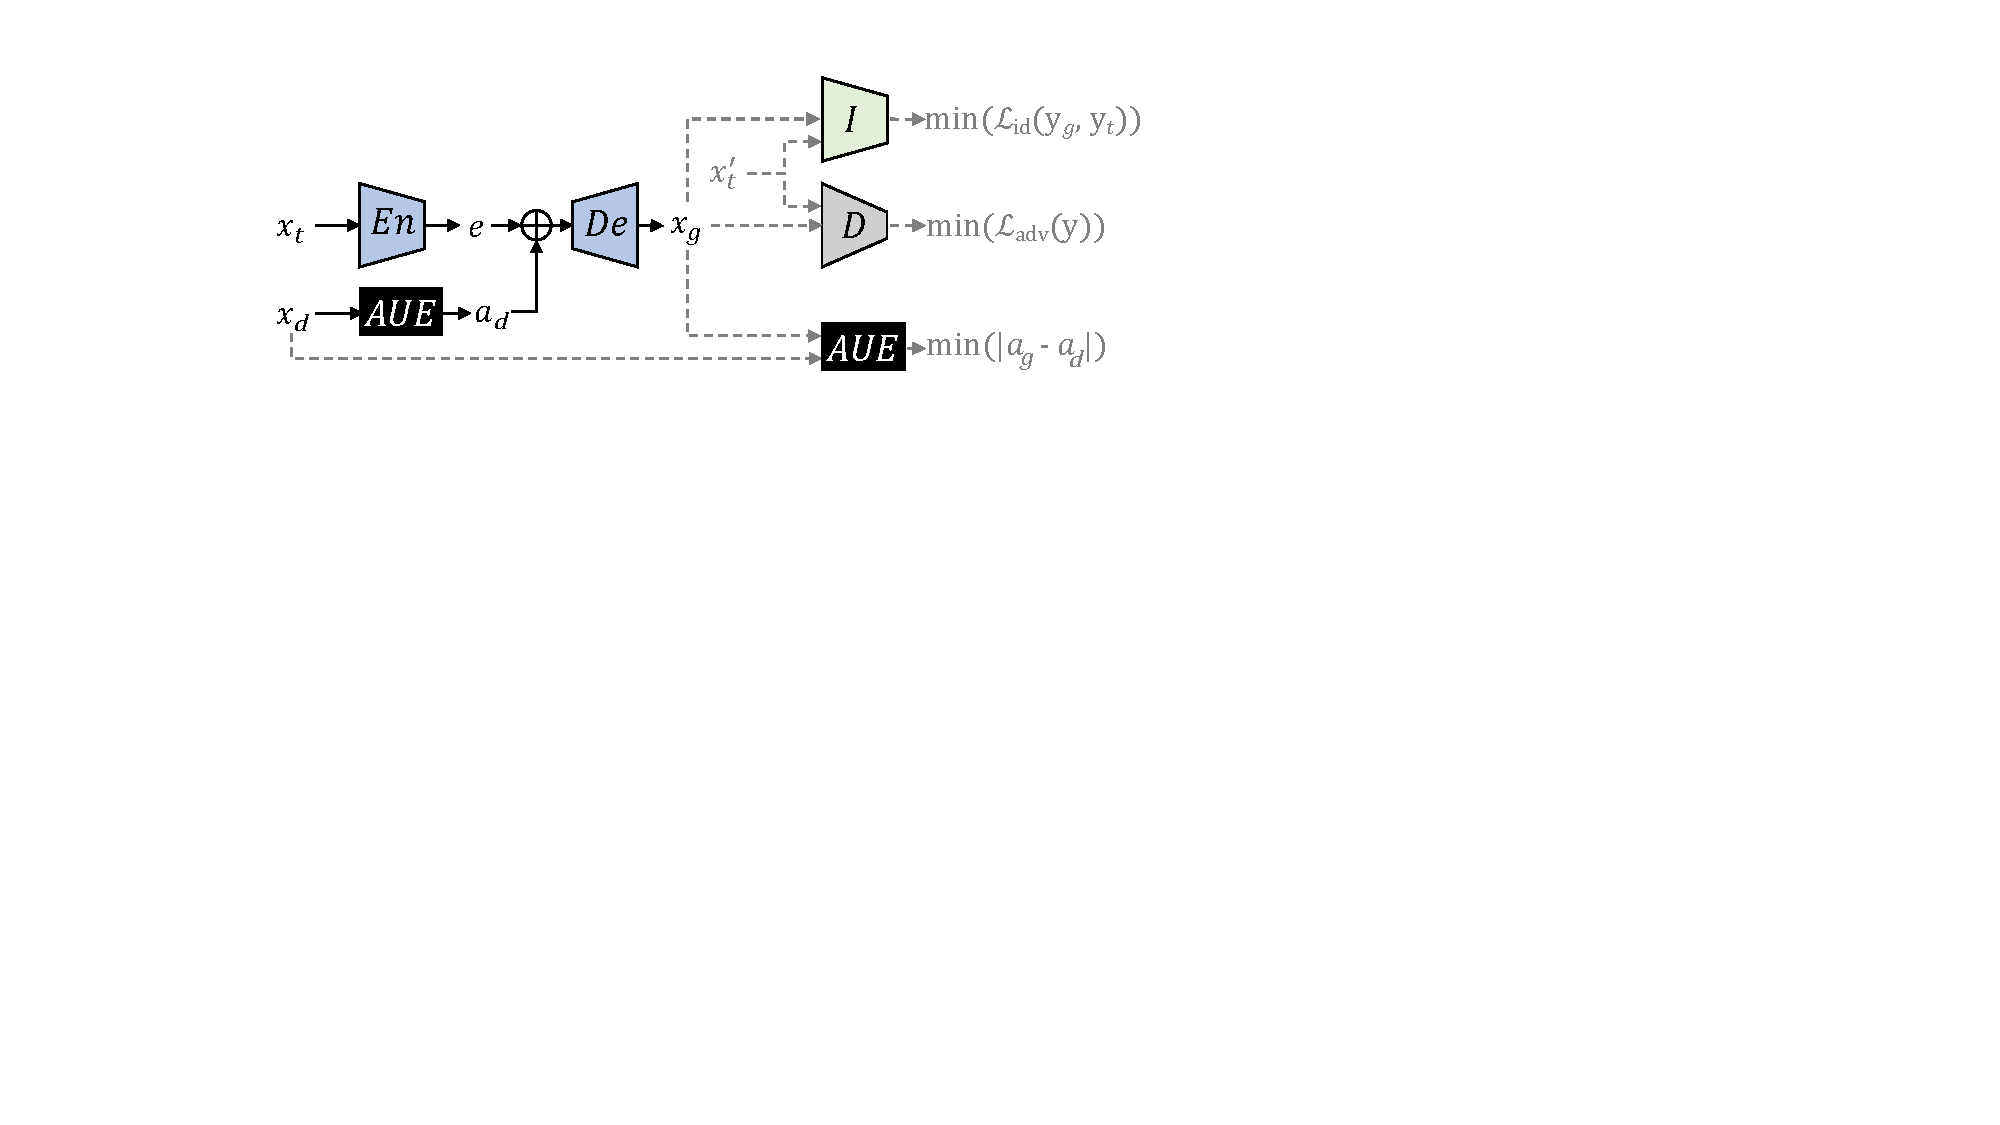
\includegraphics[width=.6\textwidth]{gath_aue_id_disc.pdf}
    \caption{\gls{ed}-architecture enriched with \glspl{au}, an identity
    and an realism constraint, where \(\bigoplus\) denotes concatenation,
    \(x'_t\) is a randomly chosen image with identity of the target \(t\). Grey
    paths are used solely in training, inspired by~\cite{Mirsky.2020, Pham.2018}}\label{fig:gath-aue-id-disc}
    \vspace{-1em}
\end{figure}

\section{Detection of DeepFakes}
We will focus on the detection of DeepFakes, even though there is also some research in the area of
prevention.

\subsection{Physical Approach}
A human on average blinks every two to ten seconds with a duration of \(0.1-0.4\) seconds~\cite{li_ictu_2018}.
Based on this spontaneous eye blinking would be expected in DeepFake videos.
This however is not always the case.
An exmplanation for this circumstance lies in the training data for \glspl{gan}.
As \textcite{li_ictu_2018} describe, with an exposure time of \(1/30\) of a second,
the likelyhood of being captured on a picture while blinking is around \(7.5\%\)~\cite{li_ictu_2018}.
In combination with the fact that most people might prefer pictures of them when they do not blink online,
is commonly thought to be one of the major reasons for this discrepancy~\cite{pishori_detecting_2020}.
Based on this oberservation, the frequency of blinking can be measured and result in a likelyhood of
a video being a DeepFake.

Central for this process is a preprocessing phase which includes the detection of eyes and blinking.

The next aspect is the prediction of an eyes new state, for this a \gls{lrcn}~\cite{donahue_long-term_2014} is used.
This is because blinking of human eyes displays strong dependencies to previous and next images.
The \gls{lrcn}-model enables capturing this by utilizing a combination of \glspl{cnn} and \glspl{lstm}~\cite{donahue_long-term_2014}.
The \gls{cnn} is responsible for the feature detection, in this case the eye region into dricrimitave features~\cite{li_ictu_2018,donahue_long-term_2014}.
The \gls{lstm} 

\todo{In Ictu Oculi: Exposing AI Created Fake Videos by Detecting Eye Blinking}

\subsection{Artifact-Based Approach}
The algorithms for creating DeepFakes might introduce artifacts in the resulting images.
These artifacts can be used to discover DeepFakes and lay the foundation for this type of detection.
\todo{Deepfake Video Detection throughOptical Flow Based CNN}

\subsection{Undirected Approaches}
In this approach, the focus is not on the artifacts, but on training gerneric neural networks, which can decide by themself on relevant
features which inform about whether or not an image is fake.
\todo{owards open-set identity preserving facesynthesis}

\subsection{Research Challenges}
When researching DeepFake detection, there is the challenge of having high quality data sets to train and test models on~\cite{li_celeb-df_2019}.

\section{Conclusion}
There are different approaches to dealing with \textit{DeepFakes}, some more
promising than others. We consider methods of detection to be only one part of a
possible solution since, on their own, they would possibly only lead to a race
between \glspl{nn} for the creation and for the detection of \textit{DeepFakes},
both getting more and more sophisticated. In this aspect, we agree with~\textcite{Mirsky.2020}'s
ideas that out-of-band methods for signatures of multimedia content and other
prevention mechanisms are required for a better solution. However, a sole focus
on technical solutions might also be futile. More effective might be to, at the
same time, try to adapt on a legal and society level to this new situation,
being aware of the existence of possibly false media content.


% Backmatter
% Bibliography and lists 
{\hypersetup{hidelinks}
    \printbibliography{}
    \printglossaries{}
    \listoffigures
    \listoftables
}
\appendix

%\chapter{General Todos}

\end{document}